\documentclass[11pt]{article}
\usepackage[margin=1in]{geometry}
\usepackage{fontspec}
\setmonofont[Path=../qmsve/fonts/]{DejaVuSansMono.ttf}
\usepackage{amsmath,amssymb,amsthm,mathtools,booktabs,graphicx,hyperref}
\hypersetup{hidelinks}
\emergencystretch=3em
\newtheorem{theorem}{Theorem}
\newtheorem{proposition}[theorem]{Proposition}
\newtheorem{corollary}[theorem]{Corollary}
\newcommand{\R}{\mathbb R}
\newcommand{\ket}[1]{\lvert #1\rangle}
\newcommand{\cP}{\mathcal P}
\title{Prior-Robust QSVT Filter Selection:\\Gap-Free Bias and Finite-Budget Risk}
\author{}
\date{}
\begin{document}
\maketitle
\begin{abstract}
Spectral filtering must balance conditional bias against rejected preparations
and finite measurement data. We study real QSVT filters for a specified
spectral-mean estimator with only an interval containing the minimum and a
lower bound on its initial mass; no spectral-gap promise enters selection.
A two-point bias characterization and a controlled endpoint-nulling
reduction yield an exact acceptance objective and certified polynomial
selection in a restricted restart model. We then distinguish stopping after
a fixed number of accepted readouts from stopping at a hard total budget.
For ideal circuits and finite attempts, we give the conditional mean-square
error and abstention law, and prove that the worst conditional risk is
attained on at most three energies. Applying classical inverse-binomial
moment bounds gives a computable prior-only finite-budget rule that includes
the no-computation midpoint. Analytic priors for six small Ising chains
connect the theory to a physical model. Experiments resolve sampling error,
bias floors, abstention and budget-dependent choices, with 2.28 million
sampling replicates. Finite sampling and moment-support arguments are
established tools; the contribution is their explicit spectral-risk
characterization and certified use in this fixed filter/estimator model,
not a new QSVT primitive or a general quantum advantage.
\end{abstract}

\section{Introduction}
Quantum singular-value transformation (QSVT) implements polynomial responses
of a block-encoded matrix \cite{Gilyen,Martyn}. This flexibility motivates
choosing different functions for different spectral problems. Such a choice
is useful only when the input information used to select it is available
and the preparation, normalization, readout and rejection costs are counted.
A low-degree filter with a small accepted-state error can still be an
expensive estimator if its acceptance probability is small.

We make this choice precise for one deliberately restricted, verifiable
setting: a nonadaptive real polynomial filter followed by independent
Bernoulli measurements of the normalized right Gram operator. The minimum
lies in a supplied interval, its initial mass is lower bounded, and no
gap is promised. The design must work for every finite spectrum compatible
with this information, rather than selecting a filter after examining the
true eigenvalues. The estimator is not intended to replace phase estimation
or modern ground-energy estimators in general.

Three results organize the analysis. First, the robust mean-bias condition
is equivalent to a two-energy inequality. Second, multiplying an admissible
filter by $1-x$ preserves this condition and gives an explicit acceptance
comparison with an endpoint-nulling filter. Third, endpoint nulling makes
the worst acceptance exactly the minimum target transmission times the
overlap bound. This identifies a semi-infinite linear program whose
objective directly controls worst expected restart cost. Exact continuous
feasibility certificates and corrected dual bounds then turn numerical
design into a quantitatively certified selection rule.

A second objective is needed when total executions are finite. Keeping
only a prescribed number of successful readouts leaves the stopping time
unbounded. We therefore analyze the exact ideal-circuit sampling law at a
fixed attempt budget, prove a three-energy reduction for worst conditional
MSE, and study a bound-based prior-only selection with abstention control.
This extension uses classical binomial inverse moments and moment-set
geometry, with attribution rather than claims of general statistical novelty.

\paragraph{Relation to existing filtering.}
Powers of cosine, spectral-ratio bounds, shifts and amplification already
appear in ground-state preparation \cite{Ge}. Optimal polynomial projectors
with a known isolated target are established \cite{LinTong}.
Cosine and Gaussian filtering and virtual filtered observables have also
been studied \cite{Lu,He}. Filtered quantum phase estimation explicitly
balances filter cost and overlap, considers different bases, and gives
known-center minimax constructions \cite{FQPE}. Wall-Chebyshev work analyzes
robustness to coarse energy information together with success costs
\cite{Wall}. Recent constrained QSP minimax work addresses the distinction
between sampled and continuous feasibility and connects optimization to
phase synthesis \cite{Constrained}. Linear programming, minimax design,
Bernstein subdivision and QSP synthesis are therefore background tools
\cite{Charnes,Farouki,DongPhase}, not claimed inventions here.

Our narrower contribution is the endpoint-nulling reduction with its
acceptance factor, the exact restart interpretation of the unknown-minimum
coupled constraints, and certified selections for this particular
gap-free mean estimator. Unlike a fixed-center rejection-band objective,
our constraint couples every possible target in the prior interval to
every larger possible eigenvalue. Unlike fidelity guarantees, it allows
nearby unwanted eigenvalues to remain. These differences define the task;
they do not establish superiority over existing estimators or universal
priority for all the component arguments.

\section{Information, oracle and estimator model}\label{sec:model}
Let $B=A/\alpha$, where a known $\alpha\geq\|A\|_2>0$ is part of the input,
and $G=B^\dagger B$ has eigenvalues in $[0,1]$. Let $e=\lambda_{\min}(G)$.
The supplied information is
\begin{equation}\label{eq:prior}
 0\leq e\leq u<1,\qquad p_0\geq a,\quad 0<a<1,
\end{equation}
where $p_0$ is total initial probability on the minimum eigenspace.
All other eigenvalues may be arbitrarily close to $e$. Degeneracy is
included by combining weights in the target eigenspace. There is no
assumption that the spectrum or its weights can be read classically.
The numerical generator knows them only to audit the resulting guarantees.

A real amplitude $P$ obeys $|P(x)|\leq1$ on $[0,1]$ and is nonzero on
$[0,u]$. For polynomials we choose its sign so $P>0$ there. The accepted
state has weights proportional to $p_iP(\lambda_i)^2$, success
$Z_P=\sum_i p_iP(\lambda_i)^2$, and mean
\[
 \mu_P=\frac{\sum_i p_iP(\lambda_i)^2\lambda_i}{Z_P}.
\]
For robustness let $\mathfrak I(a,u)$ denote all such finite spectra and
weights, and define
\[
 S(P)=\inf_{I\in\mathfrak I(a,u)}Z_P(I),\qquad
 P\text{ admissible at }b\iff \mu_P(I)-e(I)\leq b\quad\forall I.
\]
Success is physically implemented with amplitude $\kappa P$, for the common
margin $\kappa=19/20$, applied once to the entire polynomial. This changes
success by $\kappa^2$ and leaves conditional means unchanged.

For a degree-$n$ polynomial in $x=\lambda$, $P(s^2)$ is an even degree-$2n$
polynomial in the normalized singular value $s$. We assume an ideal
controlled singular-value signal and its inverse, with the standard QSVT
reflections available. A conservative serial implementation of real-valued
response extraction uses a controlled QSP unitary and its inverse: $4n$ signal calls
per complete filter attempt. This convention is used for every candidate.
It includes neither a hardware gate compilation nor a T-count claim.
State preparation costs $c_\psi$ query units, with serial depth $d_\psi$
specified separately if needed. The depth restriction is
$d_\psi+4n+1\leq D$; the last call performs readout. In the numerical model
we conservatively set $d_\psi=c_\psi$. Thus all methods within a given
problem obey the same full serial-query cap.

Given an accepted state, the success flag of a block-encoding of $B$ is a
Bernoulli variable of mean $\mu_P$. For total normalized Gram error $E$,
allocate $0<b<E$ to bias and $E-b$ to sampling. With
\begin{equation}\label{eq:shots}
 M(b)=\left\lceil\frac{\log(2/\delta)}{2(E-b)^2}\right\rceil
\end{equation}
independent accepted copies, Hoeffding's inequality yields
$|\widehat\mu-e|\leq E$ with probability at least $1-\delta$.
Our restart protocol discards every failed whole-filter attempt, prepares
the input again, and uses no amplitude amplification or intermediate
recycling. Its worst expected query cost is exactly
\begin{equation}\label{eq:cost}
 J(P,n,b)=M(b)\left[\frac{c_\psi+4n}{\kappa^2 S(P)}+1\right].
\end{equation}
Independence of fresh attempts justifies the geometric waiting time and
the identical conditional distribution of accepted readouts.

The right minimum singular value is
$\sigma_R(A)=\min_{\|v\|=1}\|Av\|=\alpha\sqrt e$. Clipping readout to
$[0,1]$ and taking a square root gives error at most $\alpha\sqrt E$.
For wide matrices this right minimum is zero and need not equal the
smallest entry of the thin SVD. Prior acquisition cost is an additional
common input cost, not included in the optimization; acquiring a tighter
prior adaptively is outside the model.

\paragraph{The no-computation baseline.}
Returning $u/2$ already estimates $e$ to $u/2$; returning
$\alpha\sqrt u/2$ estimates $\sigma_R$ to $\alpha\sqrt u/2$.
These strategies must be preferred whenever the requested error allows
them. Our main numerical tests impose $u>4E$, so neither midpoint solves
even the singular-value task with tolerance $\alpha\sqrt E$.
The unfiltered mean has worst bias $1-a$ and is feasible only if its
allocated bias is at least that large. These observations concern this
mean estimator, not every possible unfiltered quantum algorithm.

\section{Two-point characterization and endpoint reduction}
\begin{proposition}[Uniform mean-bias condition]\label{prop:pair}
An amplitude $P$ nonzero on $[0,u]$ is admissible at $b>0$ if and only if
for every $0\leq e\leq u$ and $e+b<x\leq1$,
\begin{equation}\label{eq:pair}
 (1-a)(x-e-b)P(x)^2\leq abP(e)^2.
\end{equation}
\end{proposition}
\begin{proof}
Necessity follows by placing mass $a$ at $e$ and $1-a$ at $x$ and
cross-multiplying the positive posterior denominator. For sufficiency,
let actual target mass be $p_0\geq a$. Equation~\eqref{eq:pair} implies
$(x-e-b)P(x)^2\leq abP(e)^2/(1-a)$ when $x-e>b$; if $x-e\leq b$, the
left side is nonpositive. Averaging over the non-target conditional
distribution gives
\[
 \sum_{i>0}p_i(\lambda_i-e-b)P(\lambda_i)^2
 \leq \frac{(1-p_0)ab}{1-a}P(e)^2
 \leq p_0bP(e)^2.
\]
This is exactly the bias inequality after cross-multiplication.
\end{proof}

For a fixed $e$ and exact mass $a$, the same averaging argument gives the
exact worst mean bias
\begin{equation}\label{eq:two-point}
 \max_{e\leq x\leq1}
 \frac{(1-a)(x-e)P(x)^2}{aP(e)^2+(1-a)P(x)^2}.
\end{equation}
Thus finite examples can attain, rather than merely suggest, the
worst-case bounds. This is a simple linear-fractional extremization;
the general principle is classical \cite{Charnes}.

\begin{theorem}[Controlled endpoint nulling]\label{thm:null}
Let $u+b<1$ and let $P$ be continuous and admissible at $b$, with $|P|\leq1$.
Then $Q(x)=(1-x)P(x)$ is admissible, $|Q|\leq1$, $Q(1)=0$, and
\begin{equation}\label{eq:null-factor}
 S(Q)\geq (1-u)(1-u-b)S(P).
\end{equation}
If $P$ has degree at most $n$, $Q$ has degree at most $n+1$ in $\lambda$.
\end{theorem}
\begin{proof}
For $x\geq e$, $0\leq1-x\leq1-e$. Multiplying
\eqref{eq:pair} by $(1-e)^2$ therefore proves the condition for $Q$.
Let $m=\min_{[0,u]}P^2>0$, attained at $e_*$. Every permitted input gives
$Z_Q\geq a(1-u)^2m$.
For $P$, use the allowed witness with masses $a,1-a$ at $e_*,1$.
Equation~\eqref{eq:pair} bounds its endpoint contribution, giving
\[
 S(P)\leq am+(1-a)P(1)^2
 \leq am\frac{1-e_*}{1-e_*-b}
 \leq am\frac{1-u}{1-u-b}.
\]
Combining the two inequalities proves \eqref{eq:null-factor}.
\end{proof}

\begin{corollary}[Cost of the restriction]\label{cor:restriction}
For the same $b,M,\kappa$, transforming a degree-$n$ filter to an
endpoint-nulling degree-$(n+1)$ filter increases the worst expected cost
by at most
\begin{equation}\label{eq:restriction-cost}
 \frac{c_\psi+4(n+1)}{c_\psi+4n}
 \frac{1}{(1-u)(1-u-b)}.
\end{equation}
The additional degree must fit the depth cap. Consequently the restriction
is quantitatively controlled, but is not cost-free at a tight cap.
\end{corollary}

\begin{theorem}[Exact restart probability after endpoint nulling]\label{thm:success}
If $P$ is continuous, $P(1)=0$ and $P>0$ on $[0,u]$, let
$\tau(P)=\min_{[0,u]}P$. Then
\begin{equation}\label{eq:success}
 S(P)=a\tau(P)^2.
\end{equation}
\end{theorem}
\begin{proof}
The target component gives the lower bound. Take a minimizer $e_*$ of
$P$ on $[0,u]$ and put mass $a$ there and the remaining mass at $1$.
This witness attains the bound exactly.
\end{proof}

The factor in Theorem~\ref{thm:null} is the main structural reason to use
endpoint-nulling polynomials. It gives a meaningful comparison to the
larger real-polynomial class while making acceptance optimization exact.
It does not compare to amplitude-amplified or adaptive filtering protocols.

\section{The polynomial selection problem}\label{sec:design}
For $n\geq1$ let $\tau_n^*(a,u,b)$ be the optimum of
\begin{align}\label{eq:lp}
 \text{maximize }&\ \tau\quad\text{over real }P\in\cP_n,\ \tau\geq0,\nonumber\\
 \text{subject to }&\ |P(x)|\leq1\quad(0\leq x\leq1),\nonumber\\
 &P(1)=0,\quad P(e)\geq\tau\quad(0\leq e\leq u),\\
 &\pm P(x)\leq
   \sqrt{\frac{ab}{(1-a)(x-e-b)}}P(e)
   \quad(0\leq e\leq u,\ e+b<x\leq1).\nonumber
\end{align}
All constraints are linear in the polynomial coefficients and $\tau$.
The square-root coefficient is fixed by the supplied prior and error.
Signed response outside the target interval is allowed.
For positive $\tau$, Proposition~\ref{prop:pair} makes these constraints
equivalent to admissibility in the endpoint-nulling class. Compactness of
bounded degree-$n$ polynomials gives attainment; an optimum of zero means
no positive uniformly accepting design is supplied at that degree.

\begin{theorem}[Restricted optimum and certified selection]\label{thm:selection}
For fixed $n,b$, the smallest worst expected cost in this class is
\begin{equation}\label{eq:optcost}
 J_n^*(b)=M(b)\left[\frac{c_\psi+4n}{\kappa^2 a(\tau_n^*)^2}+1\right].
\end{equation}
Suppose a certified feasible polynomial gives $\ell_{n,b}\leq\tau_n^*$
and a valid relaxation gives $\tau_n^*\leq U_{n,b}$. Define $J^{\rm up}$
by replacing $\tau_n^*$ with $\ell_{n,b}$, and $J^{\rm lo}$ by replacing
it with $U_{n,b}$. For any finite allocation set $\mathcal B\subset(0,E)$,
selecting the feasible $(n,b)$ with smallest $J^{\rm up}$ gives
\begin{equation}\label{eq:gap}
 \frac{J_{\rm selected}}{\min_{n\leq N,\ b\in\mathcal B}J_n^*(b)}
 \leq \frac{\min J^{\rm up}}{\min J^{\rm lo}}.
\end{equation}
This is an a posteriori approximation factor for the stated degree,
allocation, restart and readout model.
\end{theorem}
\begin{proof}
Equation~\eqref{eq:optcost} follows from Theorem~\ref{thm:success} and
monotonicity of cost in $\tau$. Every valid upper/lower transmission
bound gives the corresponding reverse cost bound. Taking minima proves
\eqref{eq:gap}. A comparison family with its own continuous certificate
may supply the selected upper bound as well.
\end{proof}

With fixed $M,b$, the cost of candidate $i$ is affine in preparation cost,
$J_i(c)=M[(c+4n_i)/s_i+1]$, where $s_i$ is its worst implemented success.
Two candidates with $s_j>s_i$ and $n_j>n_i$ exchange order at
\begin{equation}\label{eq:crossover}
 c_* =\frac{4(n_j s_i-n_i s_j)}{s_j-s_i}.
\end{equation}
Transmission intervals turn this point into a certified transition
interval: an upper cost for one candidate below a lower cost for the
other proves its ordering. This explains why maximizing acceptance alone
and minimizing degree alone need not select the same response.

\section{A filter-independent prior-width limitation}\label{sec:prior-limit}
The paired requirement also limits what any fixed response can achieve,
even without a polynomial or degree restriction. This provides a useful
early rejection test for proposed acceptance budgets.
Set $A_b=ab/(1-a)$ and $\Delta_0=b/(1-a)$. For $z\geq0$ define
\begin{equation}\label{eq:F}
 F_b(z)=\max\left(\{0\}\cup
 \left\{n\log\frac{z/n-b}{A_b}:
 n\in\mathbb N_{>0},\ z/n>\Delta_0\right\}\right).
\end{equation}
Only finitely many integers contribute.

\begin{proposition}[Exact unrestricted target transmission]\label{prop:prior}
For measurable weights $0\leq w\leq1$, positive on $[0,u]$ and obeying
the paired mean-bias condition, one has
\begin{equation}\label{eq:priorbound}
 \sup_w\inf_{0\leq e\leq u}w(e)=e^{-F_b(u)}.
\end{equation}
In particular, some permitted pure-target input has expected restart
overhead at least $e^{F_b(u)}$ for any one fixed filter.
\end{proposition}
\begin{proof}
Applying the ratio form of \eqref{eq:pair} along a partition of $[0,u]$
with step lengths $d_j>\Delta_0$ gives
$w(u)\leq\prod_j A_b/(d_j-b)$. For a fixed number $n$ of steps,
concavity of $\log(d-b)$ makes the equally spaced partition strongest,
giving the upper bound in \eqref{eq:priorbound}.
For completeness, allowing arbitrary step lengths with total length at
most $z$ gives exactly \eqref{eq:F}: leftover length can be added to a
step, and equal spacing maximizes its logarithmic attenuation. Concatenating
partitions shows that $F_b$ is superadditive; it is also nondecreasing.
Thus $w_*(x)=e^{-F_b(x)}$ satisfies
$w_*(e+d)/w_*(e)\leq A_b/(d-b)$ when $d>\Delta_0$.
For $b<d\leq\Delta_0$ the required ratio bound is at least one and
monotonicity suffices. Therefore $w_*$ is feasible on the entire support
and attains the minimum at $u$, proving equality. A pure eigenstate at
$u$ has acceptance $w(u)$, proving the restart statement.
\end{proof}

The large-width exponential rate is $r_a/b$, where
$r_a=W_0((1-a)/(a\mathrm e))$ and $W_0$ is the nonnegative Lambert branch.
Indeed, maximizing $\log((d-b)/A_b)/d$ gives
$d_*=b(1+1/r_a)$. The exponential weight $\exp(-r_a x/b)$ satisfies
the pair condition and provides a familiar imaginary-time comparison.
Equation~\eqref{eq:priorbound} is a function-level bound, not a general
quantum-query lower bound. It does not apply to algorithms that adapt the
filter after learning more about the minimum, use a different estimator,
or amplify/recycle successes. It is also not a proof that no polynomial
can attain the same value: nonanalyticity of the displayed optimizer
alone would not establish such a statement.

\section{Continuous and phase-realization certificates}\label{sec:cert}
We use Chebyshev coefficients $P(x)=\sum_{k=0}^n c_kT_k(2x-1)$.
Finite-grid linear programming and a few exchange rounds produce
candidates, but no grid result is called a continuous certificate.
All saved decimal coefficients are interpreted as exact rationals, with
$P(1)=0$ enforced algebraically. Bernstein coefficients and outward
integer subdivision at 220-bit fixed-point precision enclose the
polynomial on whole intervals \cite{Farouki}. They certify boundedness,
positive target transmission and \eqref{eq:pair} on the full
$(e,x)\in[0,u]\times[0,1]$ rectangle. Nonphysical or already-small
separations are harmless. Exact normalization by the computed global
bound is applied once to the composite polynomial.

For an upper transmission bound, pair square roots in the grid relaxation
are rounded upward to rational numbers, which weakens the constraints.
Floating solver multipliers are converted to nonnegative rational
weights. If $y$ is this vector, $r$ is its exact stationarity residual,
and $d$ is the objective vector, weak duality gives
\begin{equation}\label{eq:dual}
 d^Tz\leq y^T h+\sum_j |r_j|B_j,\qquad r=d-A^Ty,
\end{equation}
because the true coefficient bounds are $|c_0|\leq1$, $|c_k|\leq2$
for $k>0$, and $0\leq\tau\leq1$. These Chebyshev bounds follow directly
from the cosine-integral formula for their coefficients. The stationarity
correction is kept even when numerically small. Thus an imperfect solver
dual is not silently treated as an exact optimum.

The entire even polynomial $\kappa P(s^2)$ is synthesized once with
symmetric QSP using the \texttt{pyqsp} implementation of a Newton solver
\cite{Symmetric}. The signal convention is
\[
 W(s)=\begin{pmatrix}s&i\sqrt{1-s^2}\\i\sqrt{1-s^2}&s\end{pmatrix},\qquad
 U_\Phi=e^{i\phi_0Z}\prod_{j=1}^{2n}[W(s)e^{i\phi_jZ}].
\]
The desired response is $\operatorname{Im}(U_\Phi)_{00}$, obtained using
the success block of $(-iU_\Phi+iU_\Phi^\dagger)/2$. Controlled branches
implemented serially justify the $4n$ accounting. Saved phase decimals
define exact real angles. Rational Taylor remainder enclosures for each
sine/cosine, an interval polynomial recurrence for the top row of
$U_\Phi$, and Bernstein subdivision give a uniform response error
$\eta$ on the whole singular-value interval. This is stronger than a
floating grid agreement, while remaining a certificate for the ideal
signal oracle rather than a hardware error bound.

\begin{proposition}[Accepted-state error transfer]\label{prop:phase}
Let the ideal filter success probability be at least $s>0$, and let
the implemented success block differ by operator norm at most $\eta<\sqrt s$.
Then its success probability is at least $(\sqrt s-\eta)^2$ and its
accepted Gram mean differs from the ideal mean by at most
$2\eta/\sqrt s$.
\end{proposition}
\begin{proof}
The unnormalized state error is at most $\eta$. Reverse triangle
inequality proves the success bound. Normalizing changes vector error
by at most a factor $2/\sqrt s$; pure-state trace distance is no greater
than vector distance, and the expectation of $0\leq G\leq I$ changes
by at most trace distance.
\end{proof}
Our polynomial certificate reserves $0.01b$ of the bias allocation for
this transfer, and every synthesized selected response must satisfy it.
Encoding errors would also have to be included in $\eta$ before applying
the proposition. Applying a safety scale at every scalar iteration would
instead cause an avoidable exponential penalty; synthesizing the whole
polynomial once avoids that particular artifact.

\section{Numerical study}\label{sec:results}
We use $\delta=0.05$, $\kappa=0.95$ and the finite allocation grid
$b/E\in\{0.4,0.6,0.8\}$. Eight cases use
$a\in\{0.3,0.6\}$, $u\in\{0.125,0.2\}$, $E=0.025$,
$c_\psi\in\{1,32\}$ and $N=20$. Two further cases use
$a=0.6$, $u\in\{0.25,0.4\}$, $E=0.05$, $c_\psi=1$ and $N=12$.
The full serial-query caps are $c_\psi+4N+1$ for each problem.
All cases satisfy $u>4E$, excluding the prior-midpoint solution.
The parameter $c_\psi$ is a sensitivity parameter of the cost model;
we do not claim that preparing the simple matrix-audit input costs 32
queries on actual hardware.

\paragraph{Candidates and certificates.}
The comparison families are endpoint-nulling power $(1-x)^n$,
quartic-power $(1-x^2)^t$, endpoint-nulled cosine-Taylor products
$(1-x)(1-0.72x^2)^t$, and the classical low-pass Chebyshev polynomial
\[
 (1-x)\frac{T_{n-1}((2x-1-v)/(1-v))}
                  {T_{n-1}(-(1+v)/(1-v))},
 \quad v\in\{.04,.08,.16,.28,.42,.60,.78\}.
\]
The degree is always measured in $x=\lambda$ and then converted to signal
queries identically. Normalization, target positivity and bias are
certified for every reported candidate. Optimized candidates use initial
17-target/65-tail/129-support grids, with up to three exchange rounds
against denser grids. The LP design bias is $0.98b$; the continuous
polynomial certificate uses $0.99b$, leaving $0.01b$ for realization error.
The verifier can reject a gridded optimum, so the selected design is the
best continuously certified candidate among those attempted; its
optimality gap remains controlled by the independent dual lower bound.

\begin{table}[tb]
\centering\small
\begin{tabular}{rrrrrlrrr}
\toprule
$a$ & $u$ & $E$ & $c_\psi$ & $n$ & Response & $b$ & $J^{\rm up}$ & Gap \\
\midrule
0.30 & 0.125 & 0.025 & 1 & 8 & LP & 0.015 & 1.79e+08 & 9.5\% \\
0.30 & 0.125 & 0.025 & 32 & 8 & LP & 0.015 & 3.47e+08 & 9.5\% \\
0.30 & 0.200 & 0.025 & 1 & 8 & LP & 0.020 & 1.71e+09 & 23.9\% \\
0.30 & 0.200 & 0.025 & 32 & 8 & LP & 0.020 & 3.31e+09 & 16.2\% \\
0.60 & 0.125 & 0.025 & 1 & 4 & LP & 0.015 & 3.27e+06 & 21.4\% \\
0.60 & 0.125 & 0.025 & 32 & 4 & LP & 0.015 & 9.19e+06 & 3.7\% \\
0.60 & 0.200 & 0.025 & 1 & 4 & LP & 0.015 & 1.02e+07 & 7.5\% \\
0.60 & 0.200 & 0.025 & 32 & 5 & LP & 0.015 & 2.72e+07 & 5.6\% \\
0.60 & 0.250 & 0.050 & 1 & 2 & Cheb. & 0.030 & 5.1e+05 & 4.9\% \\
0.60 & 0.400 & 0.050 & 1 & 3 & LP & 0.030 & 1.98e+06 & 7.4\% \\
\bottomrule
\end{tabular}

\caption{Prior-only selections. $n$ is Gram-polynomial degree. ``LP'' is a
certified optimized polynomial; ``Cheb.'' is a certified member of the
tested Chebyshev grid. The gap is $100(J^{\rm up}/\min J^{\rm lo}-1)$,
relative to the endpoint-nulling class, degree cap and finite allocation
grid, not to all quantum estimators.}
\label{tab:selection}
\end{table}

The selections have certified cost factors between $1.0372$ and $1.2394$
relative to the restricted optimum lower bound. Most selected responses
come from the coupled LP, but the $a=0.6,u=0.25,E=0.05$ case selects the
tested Chebyshev response instead. Thus the implementation does not
automatically prefer the newly optimized family. Power and Chebyshev
candidates are certified in all ten cases. No quartic-power or
cosine-Taylor candidate passed the requirements within the searched
degree/parameter grid in these harder cases; this is recorded as absence
of a certified candidate, not a proof of impossibility for all tunings.
Relative to the selected upper costs, the tested power upper costs range
from approximately $1.44$ to $4.36$ times as large. These are comparisons
of guaranteed costs in the common model, not empirical runtime speedups.

\begin{figure}[tb]
\centering
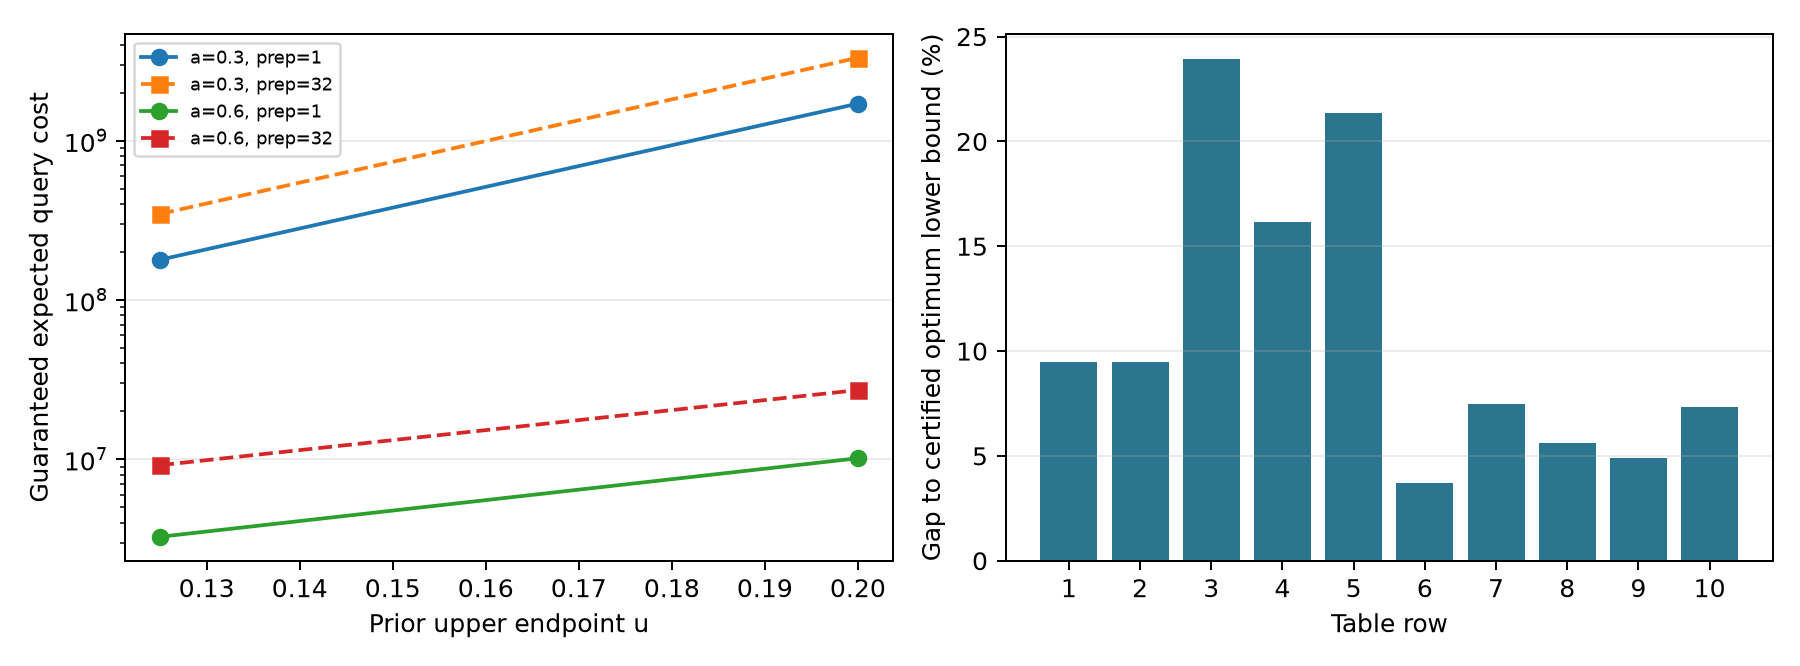
\includegraphics[width=\linewidth]{../../figures/selection_costs.png}
\caption{Guaranteed expected query costs and a posteriori gaps for the
main cases. Different preparation costs are separate specified problems;
all candidates within each problem share its cap and oracle accounting.}
\label{fig:costs}
\end{figure}

\paragraph{A preparation-cost-dependent switch.}
For $a=0.6,u=0.2,E=0.025$ and $b=0.015$, preparation cost one selects
degree four, whereas preparation cost 32 selects degree five. Both use
the same accepted-copy sample count. The latter response has greater
guaranteed acceptance, enough to compensate for the additional queries
when input preparation is expensive. For the ideal polynomial responses,
exact transmission intervals give
the crossover interval reported in the supplementary numerical summary;
the central displayed guaranteed-cost crossover is approximately $12.34$
preparation-query units. This comparison concerns two fixed certified
polynomials; it is not a claim that these are the only optimal candidates
at every intermediate preparation cost.

\begin{figure}[tb]
\centering
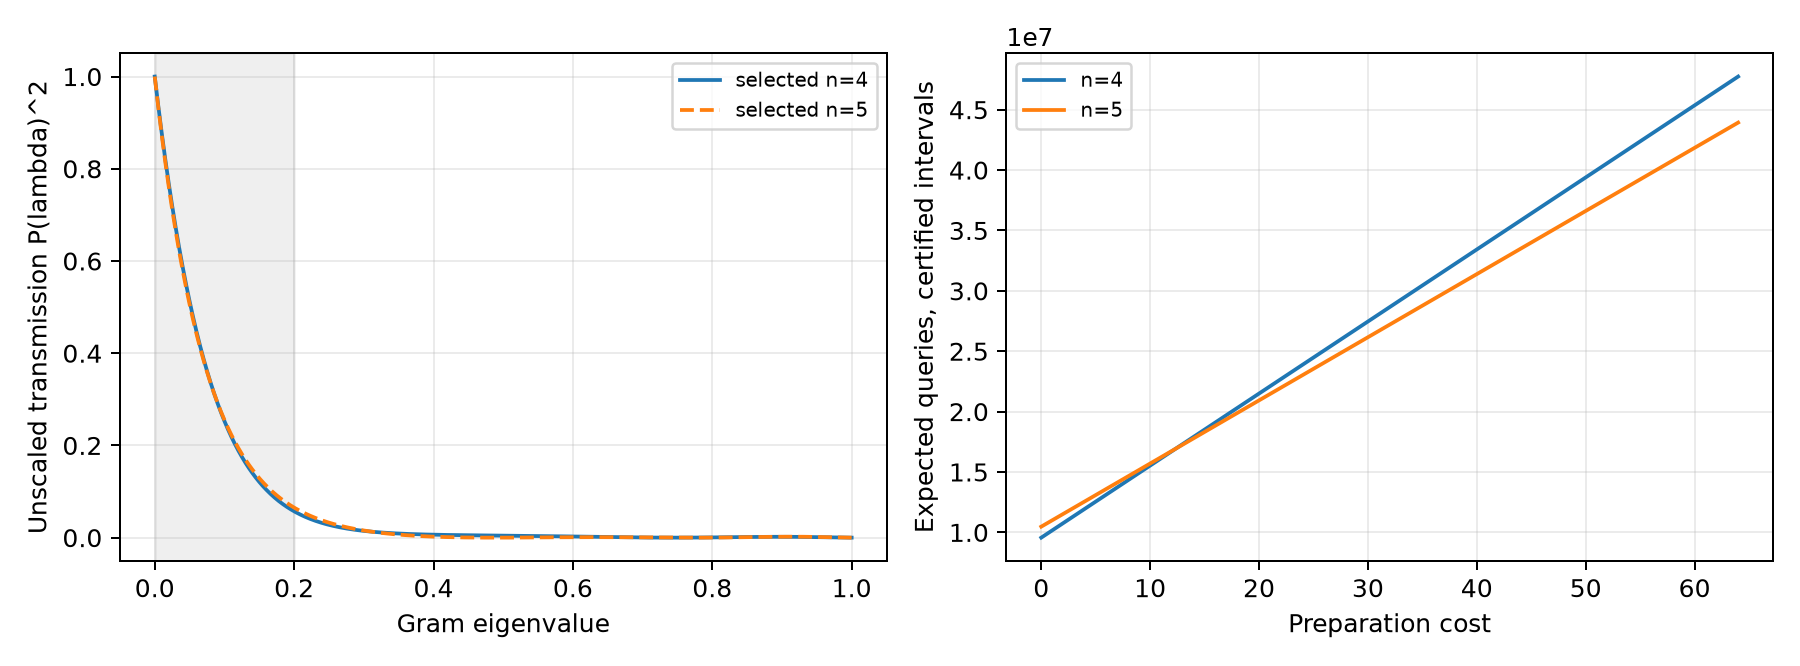
\includegraphics[width=\linewidth]{../../figures/selection_crossover.png}
\caption{Two selected responses for the same prior and bias allocation.
The shaded spectral interval is the supplied prior. Their certified
cost lines exchange order as preparation cost increases; transmission
enclosures produce the narrow bands.}
\label{fig:crossover}
\end{figure}

\paragraph{The price of prior width.}
Figure~\ref{fig:prior} compares the certified target transmissions with
the unrestricted bound of Proposition~\ref{prop:prior}. None exceeds
the function-level limit. For example, at $a=0.3$ widening the prior
from $0.125$ to $0.2$ at $E=0.025,c_\psi=1$ increases the selected
guaranteed cost from about $1.79\times10^8$ to $1.71\times10^9$ queries.
These large absolute costs do not demonstrate practicality; they
illustrate the limitations of this robust filtered-mean protocol.

\begin{figure}[tb]
\centering
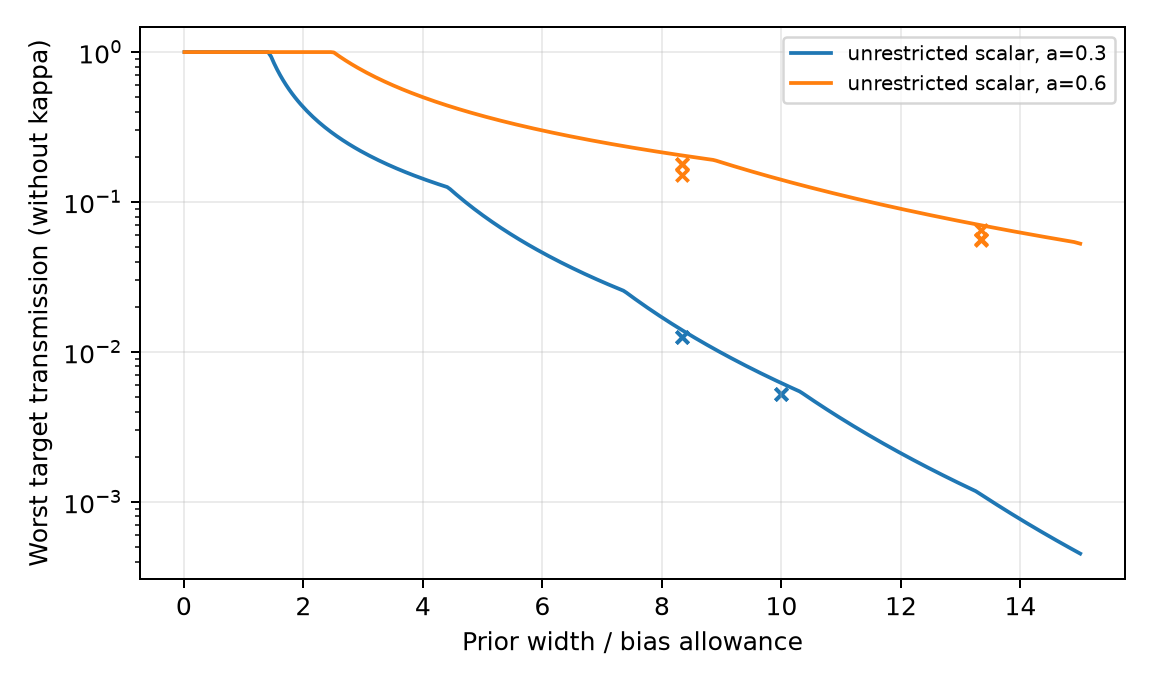
\includegraphics[width=.72\linewidth]{../../figures/selection_prior_limit.png}
\caption{The exact unrestricted target-transmission limit as a function
of prior width divided by bias allowance, and certified polynomial
transmissions (crosses). The margin $\kappa$ is excluded from both
quantities here.}
\label{fig:prior}
\end{figure}

\paragraph{Phase and matrix audits.}
All ten selected whole polynomials were synthesized successfully.
The largest certified continuous amplitude error of the saved phase
responses is $3.63\times10^{-16}$. Each satisfies the reserved mean-bias
allowance; the certified worst-success correction changes the cost
by less than a factor $1+1.4\times10^{-14}$.
These statements apply to the ideal signal convention, not to hardware
rotation synthesis or noisy block-encodings.

For each selection we also construct an eight-dimensional positive
matrix $B$ with a minimum in the supplied interval and use the fixed
computational input $\ket0$. A Householder rotation in the synthetic
generator controls its overlap promise; the estimator never receives
that rotation or the true eigenvalues for its design. One case of each
pair includes an excitation only $10^{-7}$ above the minimum.
We apply every QSP phase to the full $16\times16$ signal matrix and
explicitly form the $32\times32$ extraction unitary. The maximum
response-matrix error against the polynomial target is
$5.55\times10^{-16}$ and the maximum unitarity residual is
$6.33\times10^{-15}$. This is an exact-oracle matrix simulation, not
physical-gate compilation.

Across 1,000 held-out scalar spectral inputs (seed 20261027), the
guaranteed bias and success bounds held. A further 2,000 aggregate
Bernoulli/negative-binomial replicates for the full matrix examples
(seed 20261028) had no confidence failures at the requested error.
The confidence guarantee comes from the theorem; observing zero finite
sample failures is only a consistency check. All coefficients, phases,
input matrices, sample settings and exact certificates are included.

\section{Ideal circuits with a finite attempt budget}\label{sec:finite}
The preceding stopping rule fixes the number of accepted readouts and
controls expected cost. It does not impose a deterministic deadline.
We now hold the ideal response exactly fixed, introduce no gate noise,
and instead stop after $T\geq1$ independent whole-filter attempts.
Every attempt reserves $c_\psi+4n+1$ query units, including readout on a
rejected attempt. Thus a hard budget $B$ permits
$T_n(B)=\lfloor B/(c_\psi+4n+1)\rfloor$ attempts without overspending.
This conservative reservation is common to all candidates.

Let $w(x)$ be the implemented success weight, $z=\sum_i p_iw(\lambda_i)$
and $\mu=\sum_i p_i\lambda_iw(\lambda_i)/z$.
For the Gram experiment $w=\kappa^2P^2$.
The three outcomes of an attempt have probabilities
$1-z,z(1-\mu),z\mu$: rejection, accepted zero and accepted one.
Consequently
\[
 M\sim\operatorname{Bin}(T,z),\qquad K\mid M=m\sim\operatorname{Bin}(m,\mu).
\]
If $M=0$, the algorithm reports no estimate. Otherwise it returns
$\widehat e=K/M$, without clipping to the prior interval.
We report abstention and conditional risk separately; successful trials
are not silently substituted for a fixed number of executions.

\begin{proposition}[Finite-attempt law]\label{prop:finite-law}
For $0<z\leq1$, set $q=1-z$, $C_T(z)=1-q^T$ and
\[
 H_T(z)=\sum_{m=1}^T\binom Tm z^m q^{T-m}/m,\qquad
 h_T(z)=H_T(z)/C_T(z).
\]
Then
\begin{equation}\label{eq:finite-mse}
 \Pr(M=0)=q^T,\qquad
 R_T(z,\mu,e):=\mathbb E[(\widehat e-e)^2\mid M>0]
 = (\mu-e)^2+\mu(1-\mu)h_T(z).
\end{equation}
The failure probability at tolerance $E$, counting abstention as failure,
is exactly
\begin{equation}\label{eq:finite-failure}
 q^T+\sum_{m=1}^T\binom Tm z^m q^{T-m}
 \Pr\{\lvert\operatorname{Bin}(m,\mu)/m-e\rvert>E\}.
\end{equation}
The function $h_T$ is nonincreasing on $(0,1]$, with
$h_T(1)=1/T$ and $\lim_{z\downarrow0}h_T(z)=1$.
\end{proposition}
\begin{proof}
Condition on $M=m>0$. The sample mean has mean $\mu$ and variance
$\mu(1-\mu)/m$. Averaging its squared error proves
\eqref{eq:finite-mse}; conditioning the error event proves
\eqref{eq:finite-failure}. The positive-binomial probabilities form an
exponential family in $\log(z/(1-z))$. Differentiating a finite sum gives
\[
 h_T'(z)=\frac{\operatorname{Cov}(1/M,M\mid M>0)}{z(1-z)}
 =\frac{1-h_T(z)\mathbb E[M\mid M>0]}{z(1-z)}\leq0,
\]
where Jensen's inequality gives the last step. The endpoint limits
follow from the finite sum, since at small $z$ a nonzero count is
asymptotically one.
\end{proof}

These binomial facts and inverse moments are classical
\cite{Znid,Drakakis}; we do not claim to discover shot noise or its
$1/\sqrt T$ regime. In particular, replacing $M$ by $Tz$ is not an exact
finite-sample analysis. When $Tz$ is small, conditioning on a nonempty
sample makes $h_T$ approach one, while abstention approaches one too.
As $T$ grows at fixed $z$, sampling error vanishes but the squared bias
$(\mu-e)^2$ remains. MSE and a fixed-confidence error guarantee are
different criteria; \eqref{eq:finite-failure} evaluates the latter.

\begin{corollary}[Uniform confidence at a hard deadline]\label{cor:deadline}
If $z\geq s>0$ and $0\leq\mu-e\leq b<E$ uniformly, counting abstention
as failure gives
\begin{equation}\label{eq:deadline-confidence}
 \Pr\{\text{no output or }|\widehat e-e|>E\}
 \leq\min\{1,\,2[1-s(1-e^{-2(E-b)^2})]^T\}.
\end{equation}
Thus a sufficient deterministic attempt count at confidence $1-\delta$ is
\[
 T\geq\left\lceil\frac{\log(2/\delta)}
 {-\log[1-s(1-e^{-2(E-b)^2})]}\right\rceil.
\]
\end{corollary}
\begin{proof}
For $M=m>0$, a deviation of size $E$ from $e$ requires one of size
at least $E-b$ from $\mu$. Hoeffding bounds its probability by
$2e^{-2m(E-b)^2}$. At $m=0$, the same expression is two and hence
upper bounds the failure indicator. Average over the binomial count
and use $z\geq s$ in its generating function.
\end{proof}
This is a standard concentration/PGF consequence, not a new concentration
inequality. It translates a supplied bias/success certificate to a
hard-deadline confidence statement, which the expected-cost stopping
analysis alone does not provide.

\begin{theorem}[Three-energy reduction for conditional risk]\label{thm:three}
Fix $T$, $a$, $u$, and a continuous weight $0\leq w\leq1$ that is
positive on $[0,u]$. The maximum of \eqref{eq:finite-mse} over all finite
compatible spectra and initial weights is attained by a measure
\begin{equation}\label{eq:three}
 a\delta_e+(1-a)\{\theta\delta_x+(1-\theta)\delta_y\},
 \quad 0\leq e\leq u,\quad e\leq x,y\leq1,\quad0\leq\theta\leq1.
\end{equation}
Repeated energies are allowed, so the actual target mass can exceed $a$.
\end{theorem}
\begin{proof}
For any input with minimum $e$ and target mass at least $a$, reserve mass
$a$ at $e$ and write the remainder as a probability measure $r$ on the
original finite support, including $e$ if necessary. Hold its resulting
conditional mean $\mu$ fixed. Among remainder weights minimize
$\int w\,dr$ subject to
\begin{equation}\label{eq:moment-lp}
 \int dr=1,\qquad
 \int (x-\mu)w(x)\,dr(x)
 =\frac{a}{1-a}(\mu-e)w(e),\qquad r\geq0.
\end{equation}
The original measure is feasible. This finite linear program has an
optimal basic solution with at most two positive remainder weights,
because it has at most two independent equality constraints. The new
input preserves $\mu$, decreases $z$, and therefore cannot decrease
$R_T$ by Proposition~\ref{prop:finite-law}. It has at most three energies.
Conversely every measure in \eqref{eq:three} is allowed. The parameter
set in \eqref{eq:three} is compact and $z\geq a\min_{[0,u]}w>0$, so its
continuous risk attains its maximum.
\end{proof}

This is a task-specific application of established moment-set and
basic-solution arguments \cite{Winkler,Pinelis}. It supplies an exact
low-dimensional characterization for this finite-risk objective, rather
than equating the separate worst bias, variance and acceptance witnesses.
It does not assert that three energies are always necessary, or that the
same reduction holds for the lattice-valued failure probability in
\eqref{eq:finite-failure}, a clipped estimator, or a different stopping rule.

\paragraph{A computable uniform selection bound.}
Suppose $z\geq s>0$ and $0\leq\mu-e\leq b$ uniformly. With
$v_b=t_b(1-t_b)$, $t_b=\min\{u+b,1/2\}$, one has
\begin{equation}\label{eq:finite-upper}
 R_T\leq b^2+v_bh_T(s),\qquad
 \Pr(M=0)\leq(1-s)^T.
\end{equation}
For endpoint-nulling polynomials the abstention bound is attained at the
minimum target transmission and the upper endpoint. The MSE bound need
not be attained, since its separate worst quantities can be incompatible.
To evaluate a rigorous upper bound without summing $T$ terms, put
\[
 A_T=\frac{1-(1-s)^{T+1}}{(T+1)s},\quad
 B_T=\frac{1-[1+(T+1)s](1-s)^{T+1}}{(T+1)(T+2)s^2}.
\]
Then
\begin{equation}\label{eq:inverse-upper}
 h_T(s)\leq\min\left\{1,
 \frac{A_T+3B_T-\frac52(1-s)^T}{1-(1-s)^T}\right\}.
\end{equation}
Indeed, $1/m\leq1/(m+1)+3/[(m+1)(m+2)]$ for $m\geq1$;
the full binomial expectations of these shifted inverse powers are
$A_T,B_T$, and removing $m=0$ subtracts $5(1-s)^T/2$.
All inputs in the implementation are rational. Directed 180-bit repeated
squaring encloses powers in \eqref{eq:inverse-upper}; numerical quadrature
is used only for auditing the exact law, never for certified selection.

For a finite candidate catalog, minimize this certified risk bound at
$T_n(B)$ subject to certified abstention at most $0.05$.
Include the deterministic prior midpoint, whose worst MSE is $u^2/4$
and whose abstention probability is zero. This gives a prior-only
finite-budget rule that can select no quantum work at small budgets.
It is optimal only for the computed bound within the supplied catalog,
not a new globally optimal quantum estimation algorithm.
The resource cautions of postselected metrology remain applicable
\cite{Combes}: conditional precision alone is not an advantage if the
discarded executions are omitted.

\section{Physical application and finite-sampling experiments}\label{sec:physical}
We use open transverse-field Ising chains,
$H=-\sum_{i=1}^N X_i-J\sum_{i=1}^{N-1}Z_iZ_{i+1}$,
with initial state $\ket+^{\otimes N}$. Ising filtering is an established
benchmark \cite{QETU}; the application name is not a novelty claim.
The six cases have $N\in\{4,6,8\}$ and
$v=(N-1)J\in\{0.4,0.8\}$, so $J$ is not fixed as size changes.

\paragraph{Analytic input promises, before diagonalization.}
Let $\Delta=2-v$, $t^2=v^2/(N-1)$ and $d=t^2/\Delta$.
The unperturbed product state has energy $-N$, its orthogonal block
obeys $QHQ\succeq(-N+\Delta)Q$, and
$\|QV\ket+^{\otimes N}\|^2=t^2$: different bonds flip different pairs
in the $X$ basis. For a ground state $c\ket+^{\otimes N}+q$,
the variational bound $E_0\leq-N$ and the orthogonal block equation give
\[
 q=-(QHQ-E_0)^{-1}QV\ket+^{\otimes N}c,\quad
 -N-E_0\leq t^2/\Delta,\quad \|q\|\leq(t/\Delta)|c|.
\]
Thus $L=-N-d\leq E_0\leq U=-N$ and
$a=1/(1+t^2/\Delta^2)$ is a valid overlap lower bound.
With $R=N+v$, set $G=(H-LI)/(R-L)$, $u=d/(R-L)$ and $E=u/8$.
The physical tolerance is $d/8$, four times smaller than the prior
midpoint's worst error $d/2$. No true spectrum enters these promises.
Diagonalization is performed only after selection, to audit the result.
This promise derivation uses the known unperturbed gap; the weak-coupling
experiment is not evidence of an advantage specific to gap-free inputs.

\paragraph{Hamiltonian implementation convention.}
To apply the scalar theory to energy rather than a Gram minimum, assume
an ideal normalized Hermitian signal for $Y=2G-I$.
If $P(x)=\sum c_kT_k(2x-1)$ then
$F(y)=P((y+1)/2)=F_{\rm even}(y)+F_{\rm odd}(y)$.
Boundedness of $F$ implies boundedness of each parity part on $[-1,1]$.
Separate QSP realizations with margin $0.95$, Hermitian extraction and
LCU averaging give amplitude $0.475P(G)$. We include this factor of
one half in all nontrivial filtered application responses. The unfiltered
baseline omits extraction and has success probability one. Serial signal calls
are at most $4n$; preparation cost is the sensitivity choice $c_\psi=N$.
It is not a measured gate depth. Direct Pauli LCU for $Y$ has coefficient
norm $(2R+|R+L|)/(R-L)$, generally greater than one. The cost of realizing
the normalized signal from that LCU is not included. Consequently the
application compares an ideal oracle model, not physical gate resources.
A one-query Hadamard test on the controlled encoding of $Y$ has outcome
probability $(1+\langle Y\rangle)/2=\langle G\rangle$, supplying the
Bernoulli energy readout without assuming a free square-root Hamiltonian.

\paragraph{Application sanity check.}
At $N=4,v=0.8$, the initial energy bias is $0.053411$, above the tolerance
$0.022222$. The original selected degree-seven filter reduces the ideal
bias to $0.000368$. All six original application cases meet their bias
targets. Compared with selected guaranteed costs, the tested Chebyshev
cost factors are $1.001$--$1.173$; the three certified power cases have
factors $5.03$--$19.02$, and the other three lack a certified candidate
within the tested cap. These are finite parameter searches, not exhaustive
optimizations of the named families. Absolute costs remain large.
Saved original application phases have continuous amplitude error bounds
at most $2.04\times10^{-16}$. The following sampling study instead treats
the target polynomial itself as exact, as required by the ideal-circuit
assumption, and adds only finite measurement randomness.

\paragraph{Finite-budget catalog and reproducibility.}
For each physical prior, retain the original certified family candidates
and add LP candidates at biases
$b/u\in\{1/32,1/16,1/8,1/4,1/2\}$ and degrees
$n\in\{1,2,3,4,5,6,8,10,12,16\}$, with design/certificate margins
$0.98b,0.99b$. Failed continuous certificates are excluded.
Add the unfiltered mean and prior midpoint as baselines.
The six catalogs contain respectively $27,27,24,20,19,15$ responses
including the unfiltered mean; the midpoint is a separate option.
For each $B\in\{10^2,10^3,\ldots,10^9\}$ select by
\eqref{eq:finite-upper}--\eqref{eq:inverse-upper}, with abstention at
most $0.05$. All choices use priors only. There are 48 budget conditions;
21 select the prior midpoint. The rule changes degree and bias allocation
as the budget increases, rather than assuming the original expected-cost
choice is optimal for the new objective.

\begin{figure}[tb]
\centering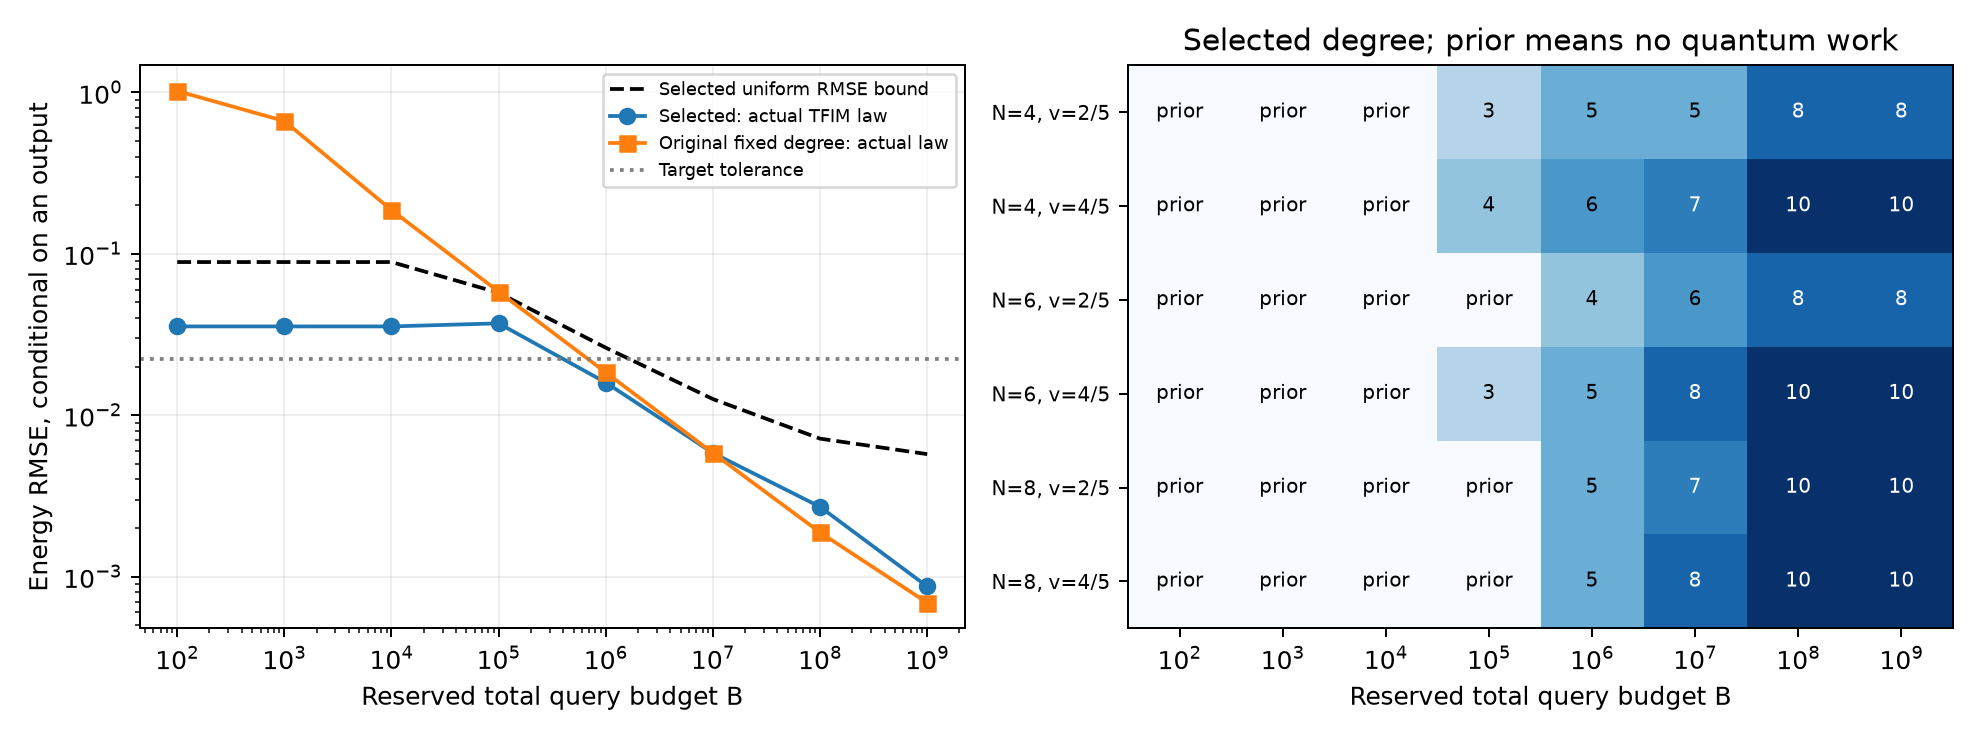
\includegraphics[width=\linewidth]{../../figures/finite_budget.png}
\caption{Ideal finite-budget selection. Left: four-spin $v=0.8$ case;
the black curve is a uniform RMSE bound, while colored curves are exact-law
numerical audits on that physical input. Right: selected degrees across
six priors; ``prior'' means no quantum work. A better uniform bound need
not give smaller actual risk on every individual spectrum.}
\label{fig:finite-budget}
\end{figure}

The three-energy reduction is checked independently on 100 random
21-energy inputs. Solving the moment LP preserves the conditional mean,
does not increase acceptance and does not decrease conditional MSE;
every reduced support has at most three energies. The largest observed
risk increase is $3.95$ times. This is a numerical check of a proved
reduction, not a certified global maximization over continuous spectra.

\paragraph{Finite counts, confidence and the bias floor.}
For the original degree-seven response at $N=4,v=0.8$:
\begin{center}\small
\begin{tabular}{rrrr}
\toprule
$B$ & conditional energy RMSE & no output & tolerance failure\\
\midrule
$10^2$ & $1.021$ & $0.711$ & $1.000$\\
$10^6$ & $0.01840$ & $<10^{-12}$ & $0.2265$\\
$10^7$ & $0.005830$ & $<10^{-12}$ & $0.000157$\\
\bottomrule
\end{tabular}
\end{center}
At $10^6$ query units the RMSE is below $0.022222$, yet the probability
of missing that tolerance is about $22.65\%$. Reporting RMSE alone would
therefore not justify a $95\%$ confidence statement. The probabilities
come from the binomial mixture \eqref{eq:finite-failure}, evaluated
numerically with omitted count mass approximately $10^{-12}$ or less.
They are not normal approximations or rational interval certificates.

Holding three filters fixed and varying $T=10^0,\ldots,10^{12}$ shows
the sampling regime and its transition to distinct bias floors.
The degree-four, seven and ten physical energy floors are respectively
$0.000763$, $0.000368$ and $0.000157$. Increasing shots cannot remove
those floors without changing the response.
Across 114 independent simulation batches we used 20,000 independent aggregate
binomial replicates each, or 2,280,000 total. Empirical MSEs agree with
the exact-law numerical predictions, with a largest discrepancy of
$3.31$ Monte Carlo standard errors. Replacing the random accepted count
by its mean in the budget study changes the predicted MSE by factors
ranging from $0.280$ to $1.293$ in these tests.
Exact rational enumeration and arithmetic controls supply 183 additional
checks; they are distinct from the Monte Carlo consistency study.

\begin{figure}[tb]
\centering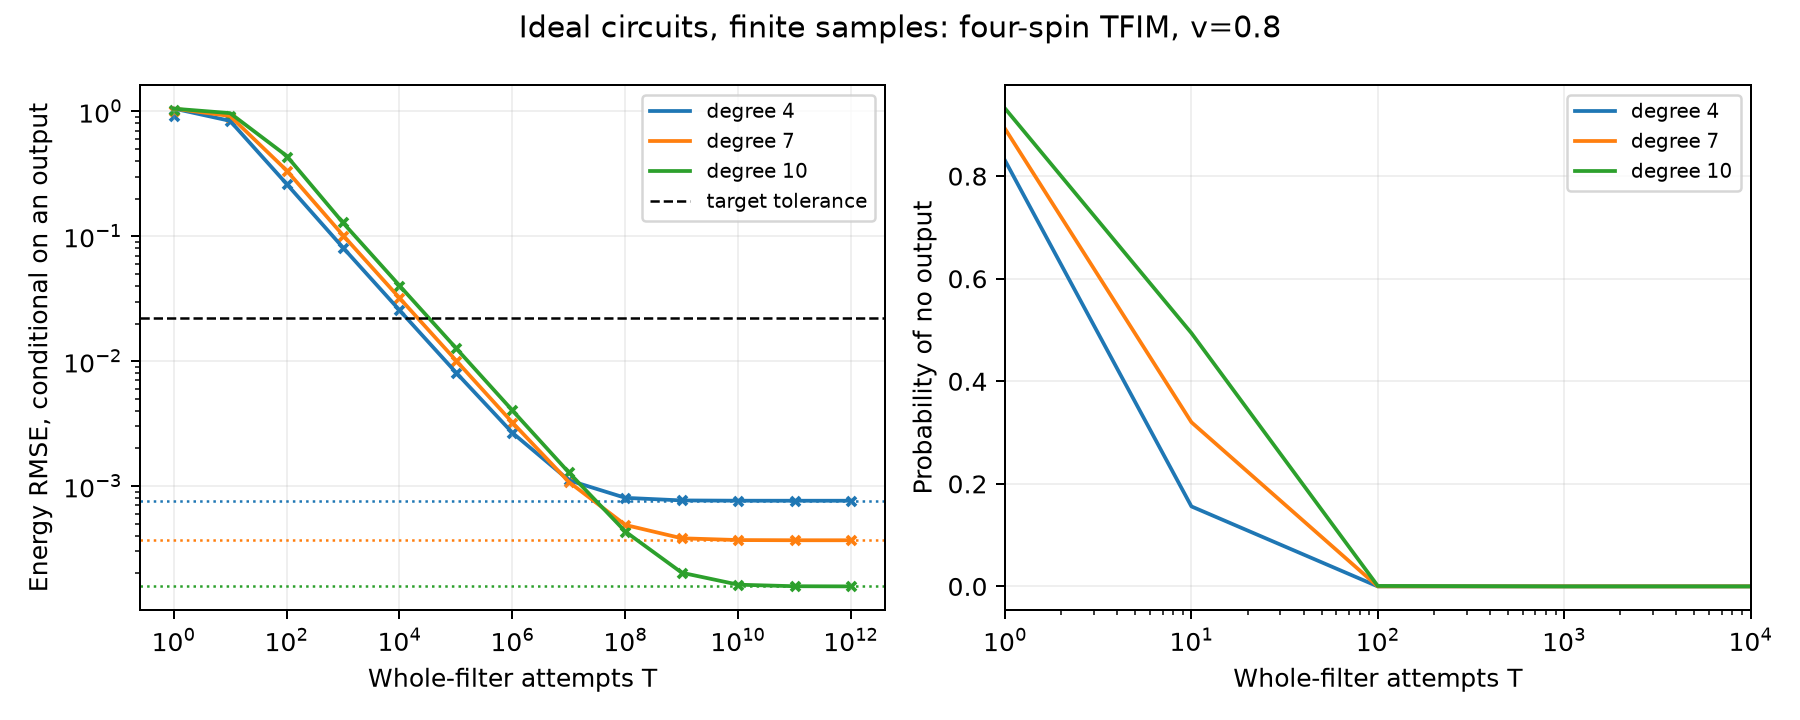
\includegraphics[width=\linewidth]{../../figures/finite_precision.png}
\caption{Ideal circuits with finite sampling on the four-spin $v=0.8$
input. Lines: exact-law numerical RMSE; crosses: Monte Carlo;
dotted levels: bias floors. Right: probability of no accepted sample.
The dashed target is a tolerance, not a confidence bound.}
\label{fig:finite-precision}
\end{figure}

The finite-budget selection is intentionally conservative. For example,
at $B=10^8$ in the representative case it selects degree ten, whose
actual RMSE is $0.00270$, while the original degree seven has $0.00188$.
The former minimizes the computed \emph{uniform bound} in the catalog;
it is not an instance-wise optimum. These small, classically tractable
Ising chains do not establish quantum advantage, thermodynamic scaling,
or superiority to QET-U or other estimators. What the extension adds is
an explicit finite-attempt accuracy/abstention objective, its spectral
reduction and an end-to-end reproducible ideal sampling test.


\section{Discussion and limitations}
The selection rule answers a concrete question with supplied prior
information: which real polynomial degree, response and finite bias
allocation minimize a guaranteed worst restart cost? The endpoint
reduction makes the restriction explicit and controls the price of using
the class in which the convex objective has an exact operational meaning.
The dual/continuous certificates distinguish proximity to a restricted
optimum from improvement over a small list of named filters.

The estimator and restart protocol are substantial restrictions.
Amplitude amplification, coherent recycling, virtual filtering,
phase-estimation-based readout and adaptive prior acquisition can change
the resource dependence. Modern QET-U and other ground-energy estimators
address different information/readout regimes \cite{QETU,Accurate}; our
results are not lower bounds on those algorithms. A supplied overlap
bound can itself be costly to obtain. Gate-level depth, error correction,
chemistry block-encodings and hardware noise are not modeled here.
Optimization over continuous bias allocations is not certified by a
finite allocation grid. Numerical near-optimality factors must always be
read with this scope attached.

The worst-case model can be conservative for a particular spectrum, and
the total costs can be large when prior width is large compared with the
bias allowance. That behavior is informative: filter flexibility alone
does not remove the price of weak prior information. The theory does not
claim a new family of optimal QSVT polynomials or a general quantum
advantage. Its contribution is the structural reduction and a
reproducible, certified answer for the specified robust selection problem.

\section{Conclusion}
We formulated prior-only gap-free filter selection for a spectral-mean
estimator with a full restart/readout query accounting. A controlled
endpoint-nulling reduction connects general real responses to a class
whose worst acceptance is exactly characterized. This yields a convex
polynomial formulation with rigorous lower and upper cost certificates,
and selected phase responses can be checked on continuous intervals.
The framework identifies when a change in preparation cost or prior
information warrants a different response, while exposing the regimes
where a fixed-filter mean estimator remains expensive.

The finite-attempt extension separates abstention, conditional MSE and
confidence. Its three-energy reduction characterizes the least favorable
risk without assuming the separate worst quantities are jointly attainable.
The numerical selection minimizes a certified bound within a finite catalog;
it need not improve actual error on every spectrum. Ideal circuits remove
hardware errors, while finite sampling and fixed-filter bias remain.

\appendix
\section{Exact arithmetic and certificate construction}
For $p(x)=\sum_{j=0}^n a_jx^j$ on $[0,L]$, its degree-$n$ Bernstein
coefficients are
\[
 b_i=\sum_{j=0}^i a_j L^j\frac{\binom ij}{\binom nj}.
\]
Because the Bernstein basis is nonnegative and sums to one, the
polynomial lies between the smallest and largest coefficients. Midpoint
subdivision uses de Casteljau averaging. The verifier rounds each lower
endpoint downward and each upper endpoint upward to integer multiples
of $2^{-220}$. Induction on subdivision proves containment.
All saved coefficient and phase decimals are exact rational inputs;
the floating optimization outputs themselves are not exact certificates.

To certify the coupled residual, write $w=P^2$ and $A_b=ab/(1-a)$.
On a box $e\in[e_0,e_1]$, $x\in[x_0,x_1]$, use $w(x)\geq0$ to bound
\[
 (x-e-b)w(x)-A_bw(e)
 \leq (x-e_0-b)w(x)-A_bw(e).
\]
The verifier encloses $xw(x)$ and $w(x)$ in the same elevated Bernstein
basis, subtracts $(e_0+b)w(x)$, and subtracts a lower bound for $A_bw(e)$.
Boxes with $x_1\leq e_0+b$ need no further check. If a box cannot be
resolved within the recorded node/depth cap, the candidate is rejected
as uncertified, even if dense-grid tests pass. This is a certificate
method, not a guaranteed optimizer or guaranteed-termination theorem.

For the phase-response recurrence write the top row as
$(P(s),i\sqrt{1-s^2}Q(s))$. One further signal/phase step gives
\[
 P_{\rm new}=e^{i\phi}[sP-(1-s^2)Q],\qquad
 Q_{\rm new}=e^{-i\phi}[P+sQ].
\]
For even signal degree the diagonal polynomial has even parity, so its
imaginary part is a polynomial in $s^2$. Rational Taylor remainders for
$\sin\phi,\cos\phi$ enclose each complex multiplication. The resulting
error polynomial in $\lambda=s^2$ is bounded with the same Bernstein
method. The stated phase bound covers a continuous interval, not only
the grid used for the separate numerical matrix check.

At $\delta=0.05$, the implementation obtains an upper rational bound
for $\log40=\log5+3\log2$ using
\[
 \log x=2\sum_{j=0}^{m-1}\frac{z^{2j+1}}{2j+1}+R_m,
 \quad z=\frac{x-1}{x+1},\quad
 0\leq R_m\leq\frac{2z^{2m+1}}{(2m+1)(1-z^2)}.
\]
It then rounds the rational shot requirement upward. Thus the integer
sample count is not based on an unchecked floating rounding at a ceiling.

\section{Formal verification scope}
\texttt{lean/Selection.lean} was checked locally with Lean 4.35.0 and
Mathlib v4.35.0 by \texttt{lake build Selection}.
\texttt{lake env lean SelectionAudit.lean} also succeeded.
The five checked scalar lemmas concern: the two-point cross-multiplication
equivalence; sufficiency for a normalized finite outside mixture with
target mass exactly $a$; preservation of the pair inequality under ordered
attenuation factors; the algebraic endpoint acceptance factor from its
two input bounds; and weak duality with a stationarity residual correction.
The audit reports only \texttt{propext}, \texttt{Classical.choice}, and
\texttt{Quot.sound}. No \texttt{sorry}, \texttt{admit}, custom axiom, or
\texttt{native\_decide} is used in those proofs.

The proof for actual target mass $p_0\geq a$, the optimization/function-space
arguments, the prior-width envelope, Bernstein algorithm, phase-realization
enclosures, matrix reduction, query implementation, and concentration
theorem are hand proofs or computational certificates, not fully formalized
Lean theorems. A workflow for the same Lean target is provided, but no
remote CI run is claimed; the reported success is local. The supplementary
verification record includes source hashes and logs.

\section{Reproducibility and scope of computation}
The finite-attempt extension adds:
\begin{itemize}
\item \texttt{finite\_sampling.py}: rational risk bounds and law audits;
\item \texttt{selection\_finite\_budget.py}: budget-based selection;
\item \texttt{selection\_finite\_precision.py}: fixed-filter shot sweeps;
\item \texttt{finite\_sampling\_figures.py}: figures and summary;
\item \texttt{check\_finite\_sampling.py}: exact-law controls;
\item \texttt{selection\_ising\_application.py}: analytic physical priors.
\end{itemize}
Saved input/source hashes link the application, budget and precision data.
The count-mixture probability sum is numerically truncated with omitted
probability approximately $10^{-12}$; its floating evaluation and the
inverse-moment quadrature are audits, not rational certificates.
The certificate calculations use exact fractions and outward fixed-point
power enclosures. The 183 controls independently enumerate small binomial
laws, compare exact reciprocal sums and check the upper bounds.

Four additional scalar lemmas in \texttt{lean/FiniteSampling.lean} were
checked locally with the same pinned toolchain, and their axiom audit
reports only \texttt{propext}, \texttt{Classical.choice}, \texttt{Quot.sound}.
They prove the pointwise inverse-count bound, risk monotonicity given
inverse-count order, variance--bias algebra, and moment-ratio preservation.
They do not formalize binomial expectations, Jensen, moment LPs or the
three-energy theorem. The corresponding local logs and source hashes
are supplied; no successful remote CI is claimed.

The source package includes these entry points:
\begin{itemize}
\item \texttt{filter\_selection.py}: design and continuous certification;
\item \texttt{selection\_qsp.py}: phase synthesis and response enclosure;
\item \texttt{selection\_matrix\_audit.py}: full block-matrix audit;
\item \texttt{selection\_figures.py}: tables, figures and summary;
\item \texttt{check\_selection\_certificates.py}: exact arithmetic controls.
\end{itemize}
Their shared arithmetic module is \texttt{selection\_certificates.py}.
The design entry point records source
hashes, base Git revision when available, rational coefficients, exact
dual bounds, certificate diagnostics, parameters and software versions.
The QSP JSON links to its design input by hash, and the matrix JSON links
to both design and phase inputs. Exact-cost rationals are provided along
with rounded displays. A complete source/hash manifest is included.

The main experiments use a small synthetic prior grid. Named baseline
parameters are searched on a finite documented grid, so comparisons are
to those certified candidates, not to every possible tuning of a named
family. Some families fail the degree/bias/certificate requirements; no
performance value is invented for them. Every main case has $u>4E$.
Earlier diagnostic cases that violated this nontriviality condition were
excluded from the reported study; they are recorded as a rejected
evaluation design in the research notes.

Author information is intentionally omitted in this review copy.
AI assistance was used for candidate derivations, drafting and numerical
implementation; the verification scopes above identify the actual checks
rather than equating generation with verification. The package has not
been uploaded or submitted to a preprint server.

\begin{thebibliography}{99}
\bibitem{Gilyen} A. Gily\'en, Y. Su, G. H. Low, and N. Wiebe, ``Quantum singular value transformation and beyond: exponential improvements for quantum matrix arithmetics,'' STOC (2019), pp. 193--204, doi:10.1145/3313276.3316366; arXiv:1806.01838.
\bibitem{Martyn} J. M. Martyn, Z. M. Rossi, A. K. Tan, and I. L. Chuang, ``Grand Unification of Quantum Algorithms,'' \emph{PRX Quantum} \textbf{2}, 040203 (2021), doi:10.1103/PRXQuantum.2.040203.
\bibitem{Ge} Y. Ge, J. Tura, and J. I. Cirac, ``Faster ground state preparation and high-precision ground energy estimation with fewer qubits,'' \emph{J. Math. Phys.} \textbf{60}, 022202 (2019), doi:10.1063/1.5027484; arXiv:1712.03193.
\bibitem{LinTong} L. Lin and Y. Tong, ``Optimal polynomial based quantum eigenstate filtering with application to solving quantum linear systems,'' \emph{Quantum} \textbf{4}, 361 (2020), doi:10.22331/q-2020-11-11-361.
\bibitem{Lu} S. Lu, M. C. Ba\~nuls, and J. I. Cirac, ``Algorithms for Quantum Simulation at Finite Energies,'' \emph{PRX Quantum} \textbf{2}, 020321 (2021), doi:10.1103/PRXQuantum.2.020321.
\bibitem{He} M.-Q. He, D.-B. Zhang, and Z. D. Wang, ``Quantum Gaussian filter for exploring ground-state properties,'' \emph{Phys. Rev. A} \textbf{106}, 032420 (2022), doi:10.1103/PhysRevA.106.032420.
\bibitem{FQPE} G. Lee, M. Kang, J. Hong, S. Fomichev, and J. Huh, ``Filtered Quantum Phase Estimation,'' arXiv:2510.04294v2 (2026).
\bibitem{Wall} M.-A. Filip and N. Fitzpatrick, ``Beyond asymptotic reasoning: the practicalities of a quantum ground state projector based on the wall-Chebyshev expansion,'' arXiv:2508.00533v3 (2026), doi:10.1088/2058-9565/ae2887.
\bibitem{Constrained} Y. Dong, J. B. Larsen, L. Lin, and R. Sarkar, ``Constrained minimax approximation for quantum signal processing,'' arXiv:2608.30937 (2026).
\bibitem{Charnes} A. Charnes and W. W. Cooper, ``Programming with linear fractional functionals,'' \emph{Naval Research Logistics Quarterly} \textbf{9}, 181--186 (1962), doi:10.1002/nav.3800090303.
\bibitem{Farouki} R. T. Farouki, ``The Bernstein polynomial basis: A centennial retrospective,'' \emph{Computer Aided Geometric Design} \textbf{29}, 379--419 (2012), doi:10.1016/j.cagd.2012.03.001.
\bibitem{DongPhase} Y. Dong, X. Meng, K. B. Whaley, and L. Lin, ``Efficient phase-factor evaluation in quantum signal processing,'' \emph{Phys. Rev. A} \textbf{103}, 042419 (2021), doi:10.1103/PhysRevA.103.042419.
\bibitem{Symmetric} Y. Dong, L. Lin, H. Ni, and J. Wang, ``Robust iterative method for symmetric quantum signal processing in all parameter regimes,'' \emph{SIAM J. Sci. Comput.} \textbf{46}, A2951--A2971 (2024); arXiv:2307.12468.
\bibitem{QETU} Y. Dong, L. Lin, and Y. Tong, ``Ground state preparation and energy estimation on early fault-tolerant quantum computers via quantum eigenvalue transformation of unitary matrices,'' \emph{PRX Quantum} \textbf{3}, 040305 (2022), doi:10.1103/PRXQuantum.3.040305.
\bibitem{Accurate} A. Dutkiewicz, T. E. O'Brien, and S. Polla, ``Accurate ground state energy estimation with noise and imperfect state preparation,'' arXiv:2603.21873v2 (2026).
\end{thebibliography}

\end{document}
